\section{Acceptance Systematics}
\label{sec:systematic}
Systematic uncertainties on signal event selections arise from uncertainties on event selections expected in simulation 
compared to the actual performance of  the detector. 
The uncertainties associated with the data - Monte Carlo scale factors 
are discussed in Section~\ref{sec:SF}
As this search is in many ways similar to the inclusive same-sign dilepton search~\cite{ssnote2011}, 
our treatment of efficiency systematics parallels the one in that analysis.
In this section, we briefly summarize those results, and
describe the uncertanities due to the b-tagging requirement.

The only new source of systematics in this analysis is from the uncertainty on the
b-jet tagging efficiency.
As already mentioned in Section~\ref{sec:bjetSF}, this uncertainty
is 4 (15)\% for jets with $\pt<240 (>240)~\GeV$.
As an illustration of the b-jet momentum distribution,
we compare them in Fig.~\ref{fig:lm9ttbar} for  \ttbar\ events (before the same-sign requirement)
and for the LM9 cMSSM SUSY benchmark point.\footnote{
The LM9 point is defined by the common scalar mass (m0) $ = 1.45$ TeV, 
the common gaugino mass (m1/2) = 175 GeV, the ratio of the Higgs expectation
values (tan$\beta)  = 10$, tri-linear coupling (A0) = 0 and the  sign of the Higgsino mass parameter ($\mu) > 0$. 
}
While most of the b-jets from \ttbar\ are below 240~\GeV, those from LM9
have a large contribution from higher momenta.
Our target searches include final states with two or more b-quark jets.
This means the efficiency to select two b-jets, as well as its uncertainty
varies among the signal final states considered
\begin{itemize}
\item same-sign top pair production, as from $Z^\prime$ exchange,
	is similar in topology to that of the opposite-sign \ttbar\ production
	and has only two b-jets in the final state with most of them with $\pt<240~\GeV$.
	The b-tagging uncertainty is then approximately 8\%
	and the corresponding per-event scale factor is $0.922 \pm 0.073$.
\item direct sbottom pair production has two b-jets in the final state
	with a large fraction of b-jets with $\pt>240~\GeV$.
	The b-tagging efficiency scale factor is still 0.922, but its uncertainty
	varies among the signal model points from as low as 8\%
	to as high as 29\%.
	This uncertainty is evaluated event-by-event and then point-by-point in the limit setting procedure.
\item gluino pair production with stops in the final states considered
	here all have four b-jets in the final state.
	Now the efficiency scale factor changes as well
	depending on the number of b-jets in the acceptance.
	This is evaluated event-by-event and point-by point in the limit setting procedure.
\end{itemize}


\begin{figure}[htb]
\begin{center}
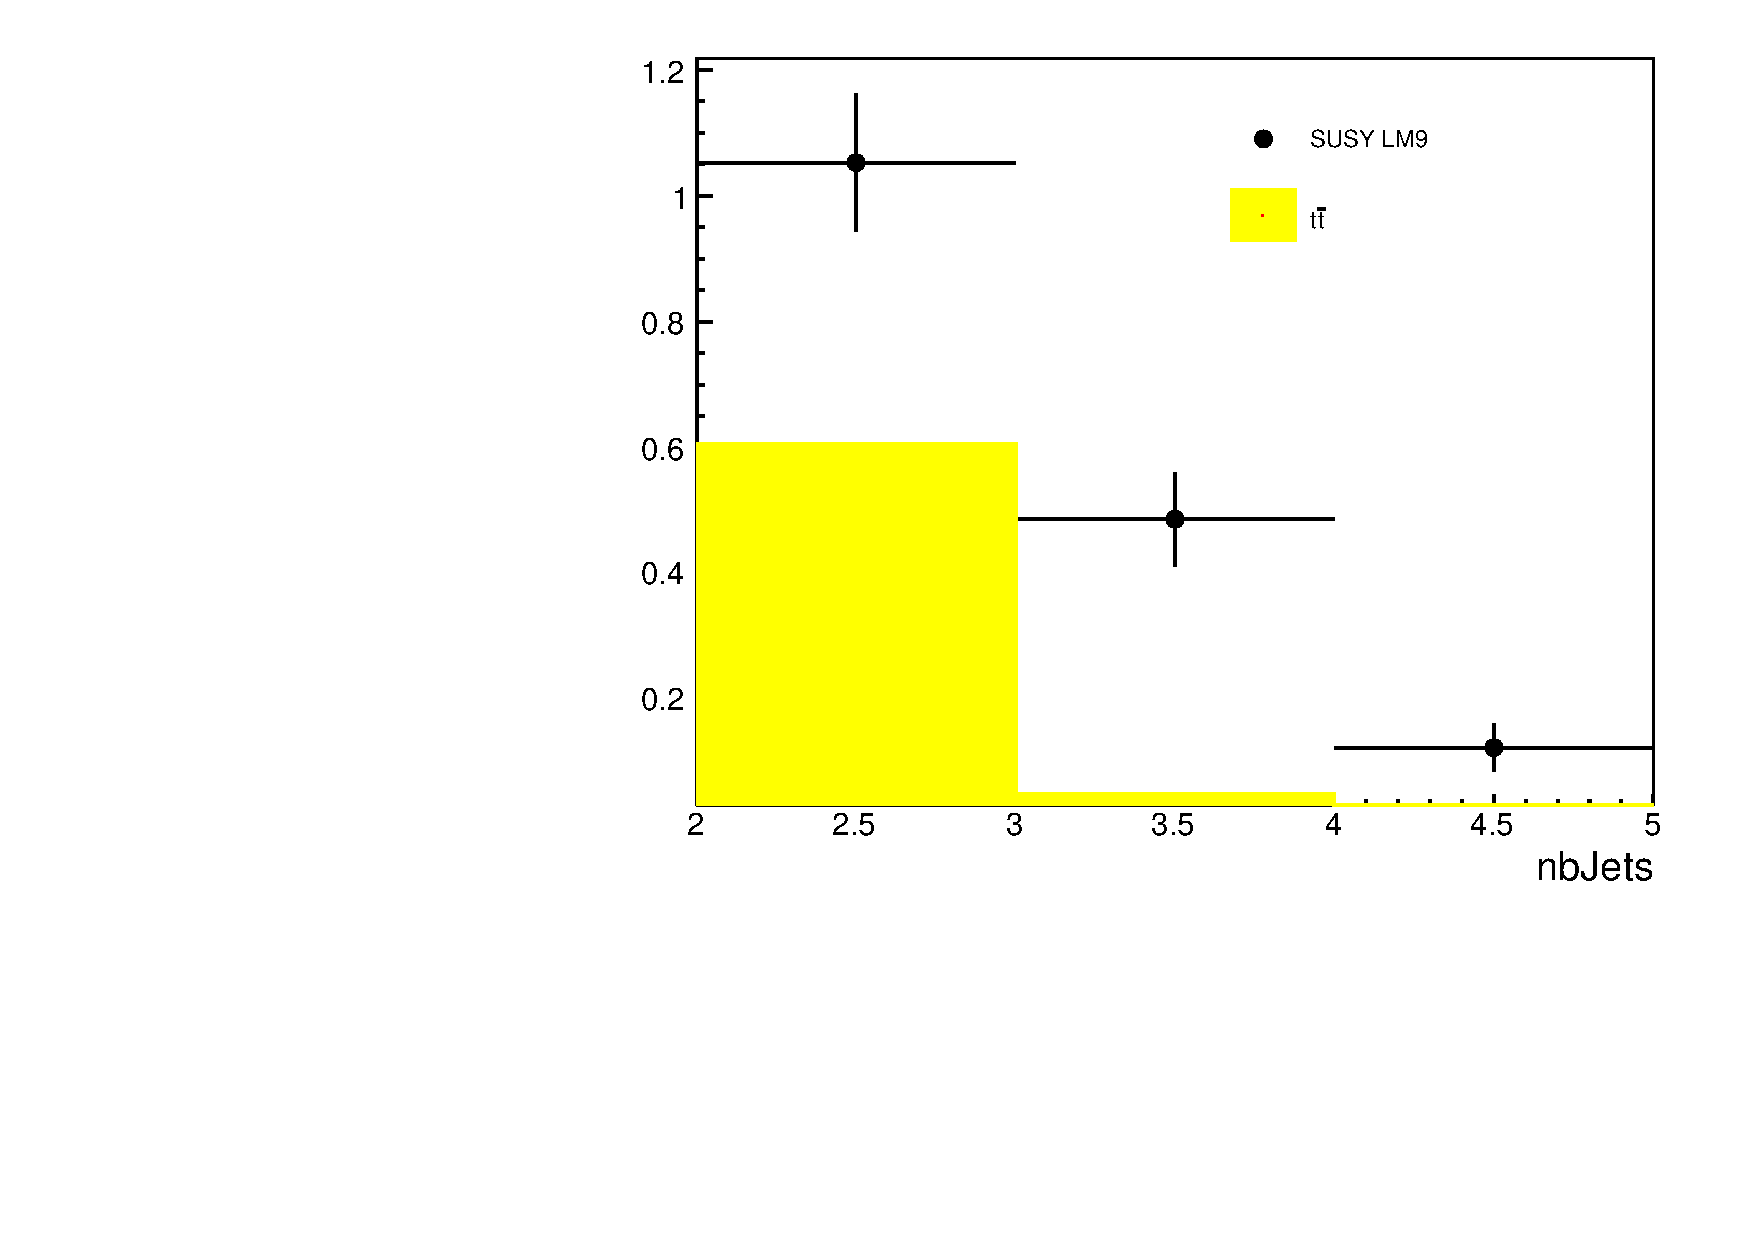
\includegraphics[width=0.48\textwidth]{figs/lm9.pdf}
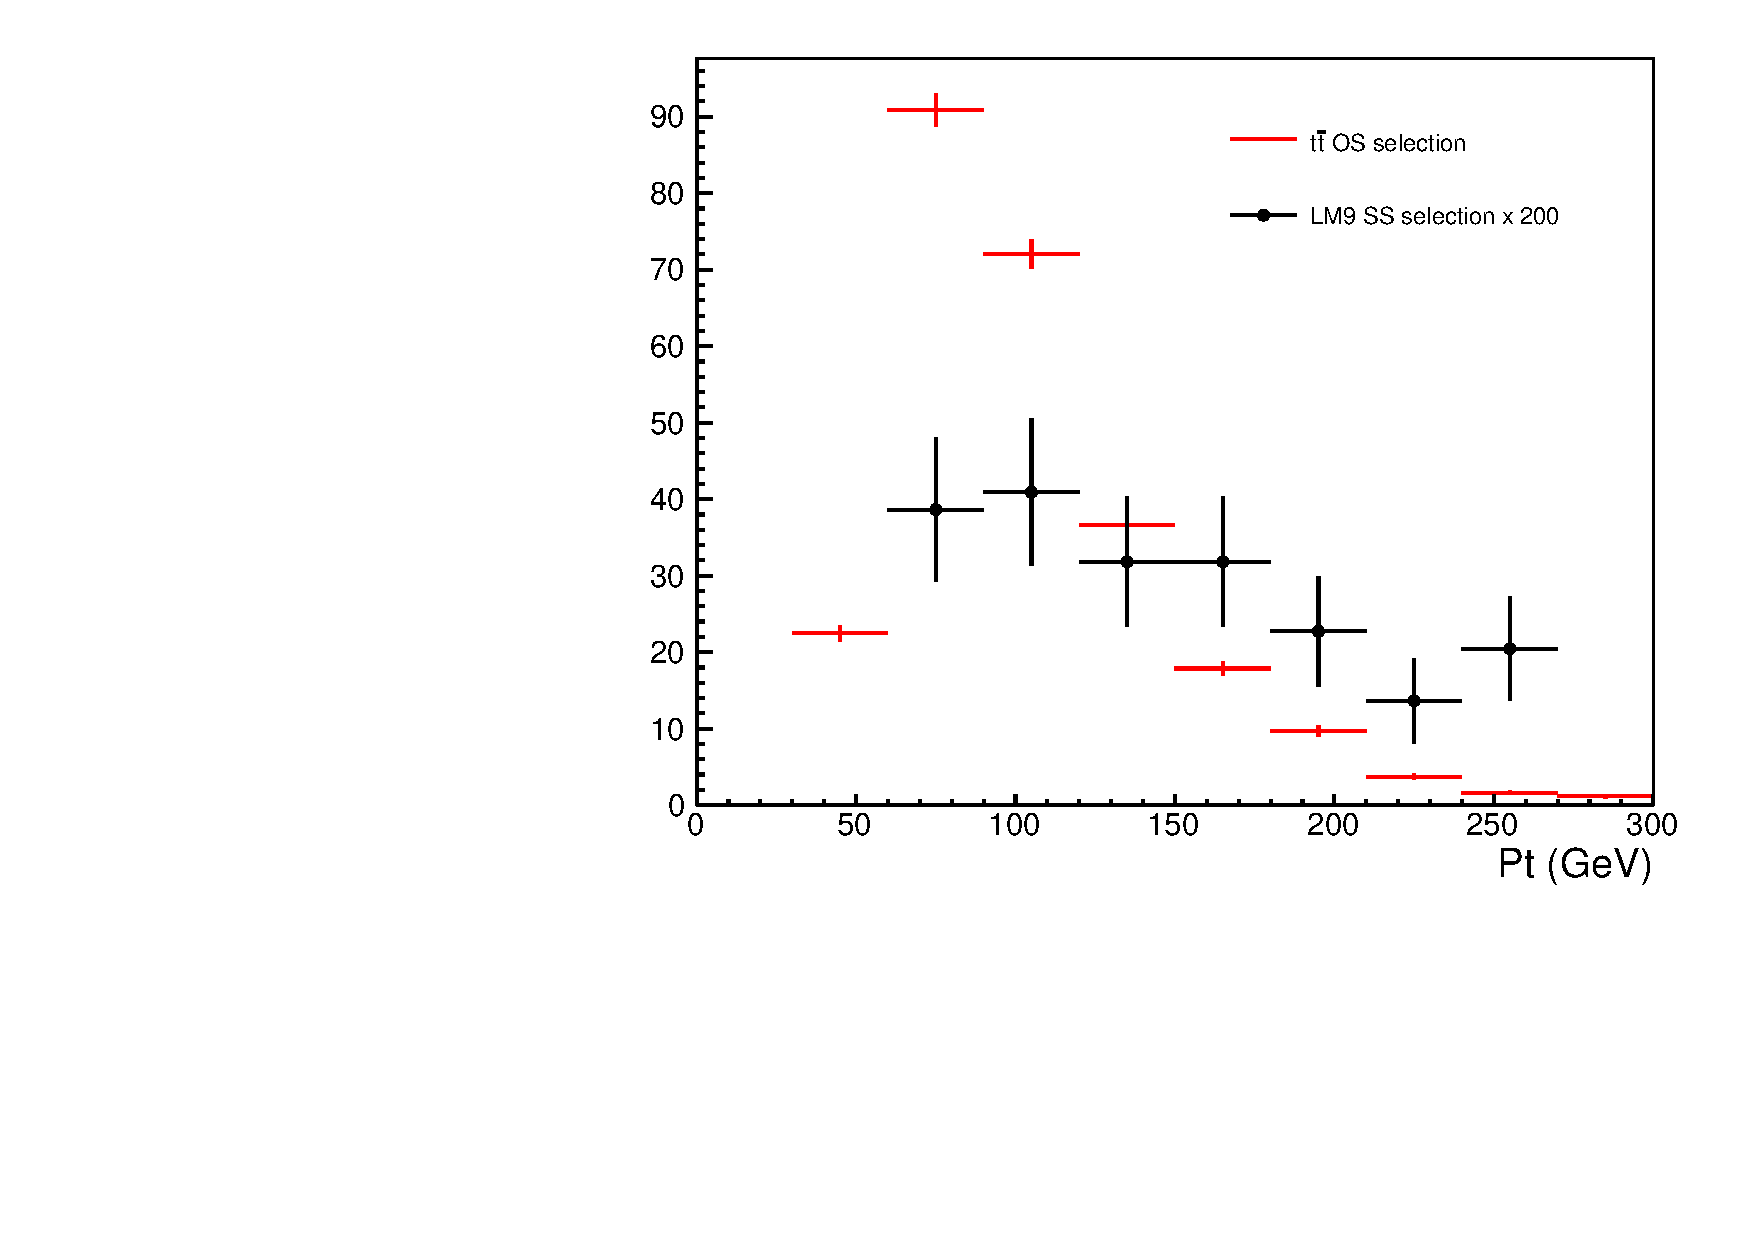
\includegraphics[width=0.48\textwidth]{figs/bjetleading.pdf}
\caption{ Differential distributions of leading b-tag jet $\pt$ for the 
LM9 benchmark point and \ttbar\ simulations.
The normalization is arbitraty.\label{fig:lm9ttbar}}
\end{center}
\end{figure}


A summary of systematic uncertainties is given in Table~\ref{tab:systSumm}.
Here the b-tagging systematics is applicable only to the same-sign top production signature.

\begin{table}[h]
\begin{center}
\caption{\small\label{tab:systSumm}Summary of systematic uncertainties on the signal selection and
expectation. 
Reported values are fractional, relative to the total cross section.
The energy scale, b-tagging, and PDF uncertainties are calculated separately in every model point.
These uncertainties quoted here are relevant to the $Z^\prime$ model.}
\begin{tabular}{lcccc}\hline
Source 					& $ee$		& $\mu\mu$		& $e\mu$	& all 	\\ \hline
Lepton selection			& 12\%		& 12\%			& 11\%		& 11\% 	\\
Energy scale				& 8\%		& 8\%			& 8\%		& 8\% 	\\
ISR/FSR and PDF				& 2\%		& 2\%			& 2\%		& 2\% 	\\
b-tag selection                         & 8\%          	& 8\%                   & 8\%           & 8\% 	\\
Total without luminosity		& 17\%		& 17\%			& 17\%		& 17\%	\\ \hline
Integrated luminosity			& 4.5\%		& 4.5\%			& 4.5\%		& 4.5\%	\\ \hline
Total 					& 17\%	 	& 17\%	 		& 17\% 		& 17\% 	\\
\hline
\end{tabular}
\end{center}
\end{table}

\subsection{Event-by-Event B-tagging scale factor and 
associated systematic uncertainty for signal regions wih $\geq$ 2 btags}
\label{sec:SF2btag}

We evaluate an event-by-event btagging scale factor ($SF_{\rm event}$) as follows:

\begin{itemize}
\item for each MC event passing the event selection we start
from the scale factors $SF_i$ associated with the two or more
tagged jets.  Note that $SF_i$ can in principle be a function 
of jet $\eta$, $\pt$, etc.  Following the btag group 
recommendations
it is taken as a constant: $SF=0.96$\cite{BTV11003, btvSyst}


\item For events with two btagged jets: $SF_{\rm event}=SF^2$.

\item For events with three btagged jets: $SF_{\rm event}=SF^3 + 3SF^2(1-SF)$.

\item For events with four btagged jets: $SF_{\rm event}=SF^4 + 4SF^3(1-SF) + 6SF^2(1-SF)^2$.
\end{itemize}

Note that the procedure above would not work if $SF>1$, but this is not an issue
since $SF=0.96$.
It also implicitely assumes that all btags are from b-quarks.  For the models under 
consideration, we have verified that the MC contribution to the acceptance from 
events that need at least one tag from $udsgc$ in order to pass the $\ge$ 2 tags 
requirements is small.  For example, in the $Z'$ model, this contribution is
only $\approx$ 4\%.  Note that the bias in $SF_{\rm event}$ due to the improper traeatment
these events is 4\% times some quantity proportional to the difference in scale 
factors between $b$-jets and $usdgc$ jets.  Therefore, it is $<<$ 4\% and we think
can be ignored.  

In order to calculate the uncertainty ($\delta SF$) on the event-by-event $SF_{\rm total}$,
we also need the single jet btagging efficiency ($\epsilon$).  
We do not need a very precise value for $\epsilon$, since the uncertainty $\delta SF$ is 
only weakly dependent on it.  We take $\epsilon = 0.643$, independent of $\pt$
and $\eta$ for jets of $|\eta| < 2.5$.  The uncertainty on $\epsilon$ is 
the same as that on the scale factors, $\delta \epsilon = 4\% (15\%)$ (relative)
for $\pt < 240$ GeV ($> 240$ GeV).
The procedure is the following:
\begin{itemize}

\item For each event passing the requirements at RECO level, we look at the status=3 information
and we calculate the total probability ($p$) of tagging two or more jets, and 
its uncertainty ($\delta p$).

\item The calculation of $p$ and $\delta p$ is based on the number of status=3 b-quarks
of $\pt > 40$ GeV and $|\eta| < 2.5$.  

\item An event with two reconstructed btags can have $<$ 2 such status=3 b-quarks.  This 
is rare and happens for example when a 39 GeV b-quark is reconstructed as a 41 GeV
b-jet.  In these cases we calculate $p$ and $\delta p$ assuming that there are 
two 40 GeV b-quarks at status=3.

\item The uncertainty associated with the event is then $(\frac{|\delta p|}{p}) SF_{\rm event}$.

\end{itemize}

The probabilities $p$ are calculated as follows ($N$ here is the number of status=3 b-quarks
and we write the equations without the assumtion that $\epsilon$ is constant):

\begin{itemize}

\item $N=2$:~~~~$p = \epsilon_1 \epsilon_2$.

\item $N=3$:~~~~$p = \epsilon_1 \epsilon_2 + \epsilon_1 \epsilon_3 + \epsilon_2 \epsilon_3 -
2\epsilon_1 \epsilon_2 \epsilon_3$.

\item $N=4$:~~~~$$p = \prod{\epsilon_i}~~~+~~~\sum_j{(1-\epsilon_j)\prod_{i \ne j}{\epsilon_i}}
~~~+~~~\sum_{j<k}{(1-\epsilon_j)(1-\epsilon_k)\prod_{i \ne j,k}{\epsilon_i}}$$



\end{itemize}

The uncertainties $\delta p$ are calculated from the equations above assuming full 
correlation between jets, {\em e.g.}, for $N=2$ we have 
$\delta p$ = $\delta \epsilon_1 \cdot \epsilon_2 + \delta \epsilon_2 \cdot \epsilon_1$, etc.


\subsection{Event-by-Event B-tagging scale factor and 
associated systematic uncertainty for signal regions with $\geq$ 3 btags}
\label{sec:SF3btag}
The treatment of Section~\ref{sec:SF2btag} for $\geq 2$ btags
is extended here to the case of $\geq 3$ btags.  
The event-by-event btagging scale factor ($SF_{\rm event}$) is evaluted
as follows:

\begin{itemize}
\item For events with 3 btagged jets $SF_{\rm event}=SF^3$.

\item For events with 4 btagged jets 
$SF_{\rm event}=SF^4 + 4SF^3(1-SF)$.

\end{itemize}

The uncertainty is calculated starting from the probability $p$ 
of having $\geq$ 3 btagged jets in events with at least $N=3$ $b$-quarks
at status=3.  This probability is

\begin{itemize}

\item $N = 3$:~~~~$p = \epsilon_1 \epsilon_2 \epsilon_3$.

\item $N = 4$:~~~~$$p = \prod{\epsilon_i}~~~+~~~\sum_j{(1-\epsilon_j)\prod_{i \ne j}{\epsilon_i}}$$

\end{itemize}

\noindent where $\epsilon_i$ is the probability of tagging the $i$-th $b$-quark.
The uncertainties $\delta p$ are calculated from the equations above assuming full 
correlation between jets, {\em e.g.}, for $N=3$ we have 
$\delta p = \sum_{i} \delta \epsilon_i \prod_{i \neq j} \epsilon_j$, etc.